\section{Data Consistency \& Quality}

\subsection{Feature Statistics Examination}

Our initial step in assessing the data's consistency and quality involved a detailed examination of the feature statistics across the entire dataset. This approach allows us to identify potential outliers, inconsistencies, and wrongly labeled audio snippets without the need to listen to each recording individually. Here's how we conducted this examination:

\subsubsection{Methodology:}

\begin{enumerate}
    \item \textbf{Descriptive Statistics}: We calculated basic descriptive statistics for each feature, including mean, median, standard deviation, and interquartile range (IQR). These metrics provide insights into the central tendency and spread of the data, helping identify features with abnormal distributions.
    \item \textbf{Outlier Detection}: By applying IQR and z-score methods, we pinpointed samples with feature values significantly deviating from the bulk of the data.
    \item \textbf{Visualization}: We utilized box plots and histograms for each feature to visually inspect their distributions. Box plots were particularly useful in spotting outliers, while histograms allowed us to observe the shape of the distributions, revealing any skewness or multimodality.
\end{enumerate}

%\begin{figure}[!ht]
%	\centering
%	\begin{minipage}{0.49\textwidth}
%		\centering
%		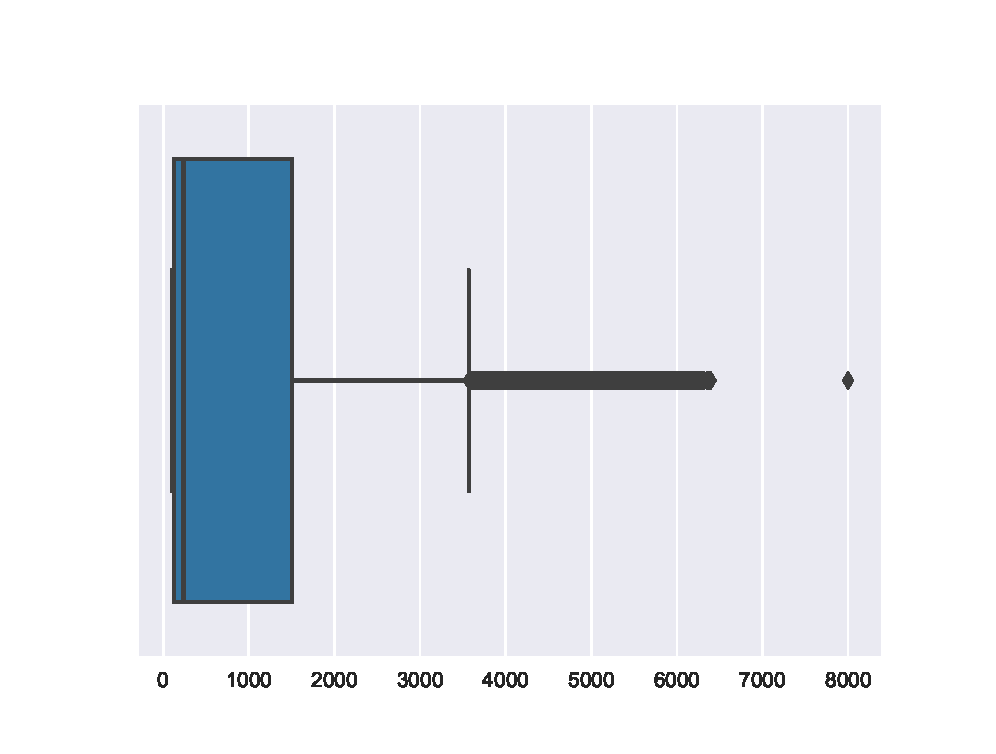
\includegraphics[scale=0.3]{fig/boxplot_skew}
%		\caption{Skewness and outliers: Feat. 173.}
%		\label{fig:Skewness}
%	\end{minipage}\hfill
%	\begin{minipage}{0.49\textwidth}
%		\centering
%		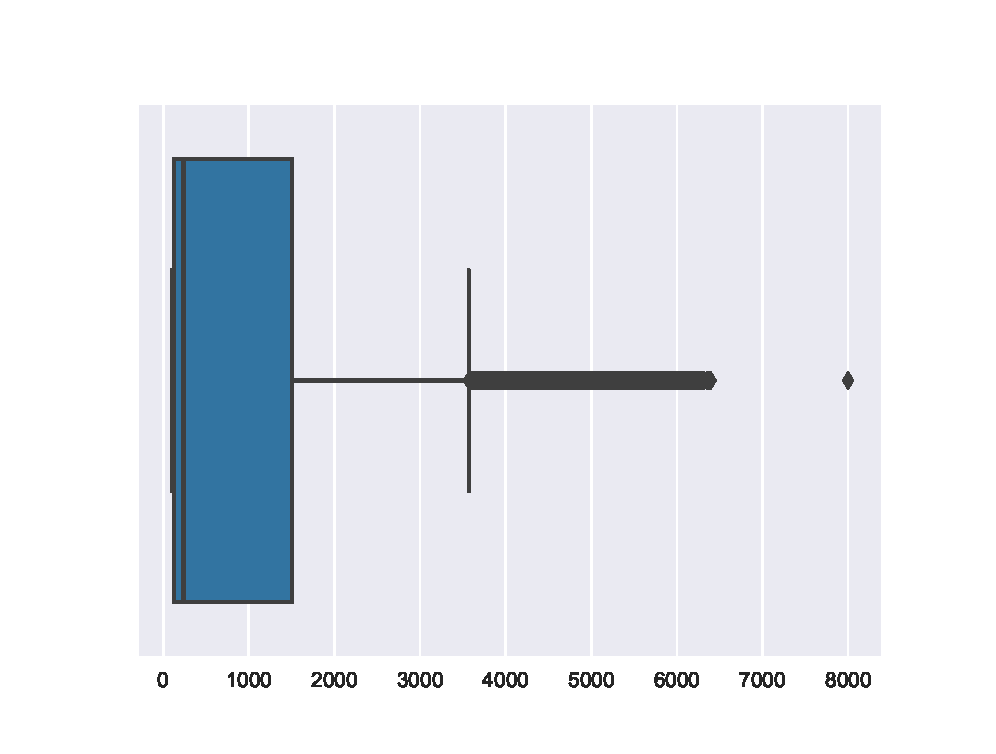
\includegraphics[scale=0.3]{fig/boxplot_skew}
%		\caption{Additional Image Description.}
%		\label{fig:additionalImage}
%	\end{minipage}
%\end{figure}

\begin{figure}[!ht]
	\centering
	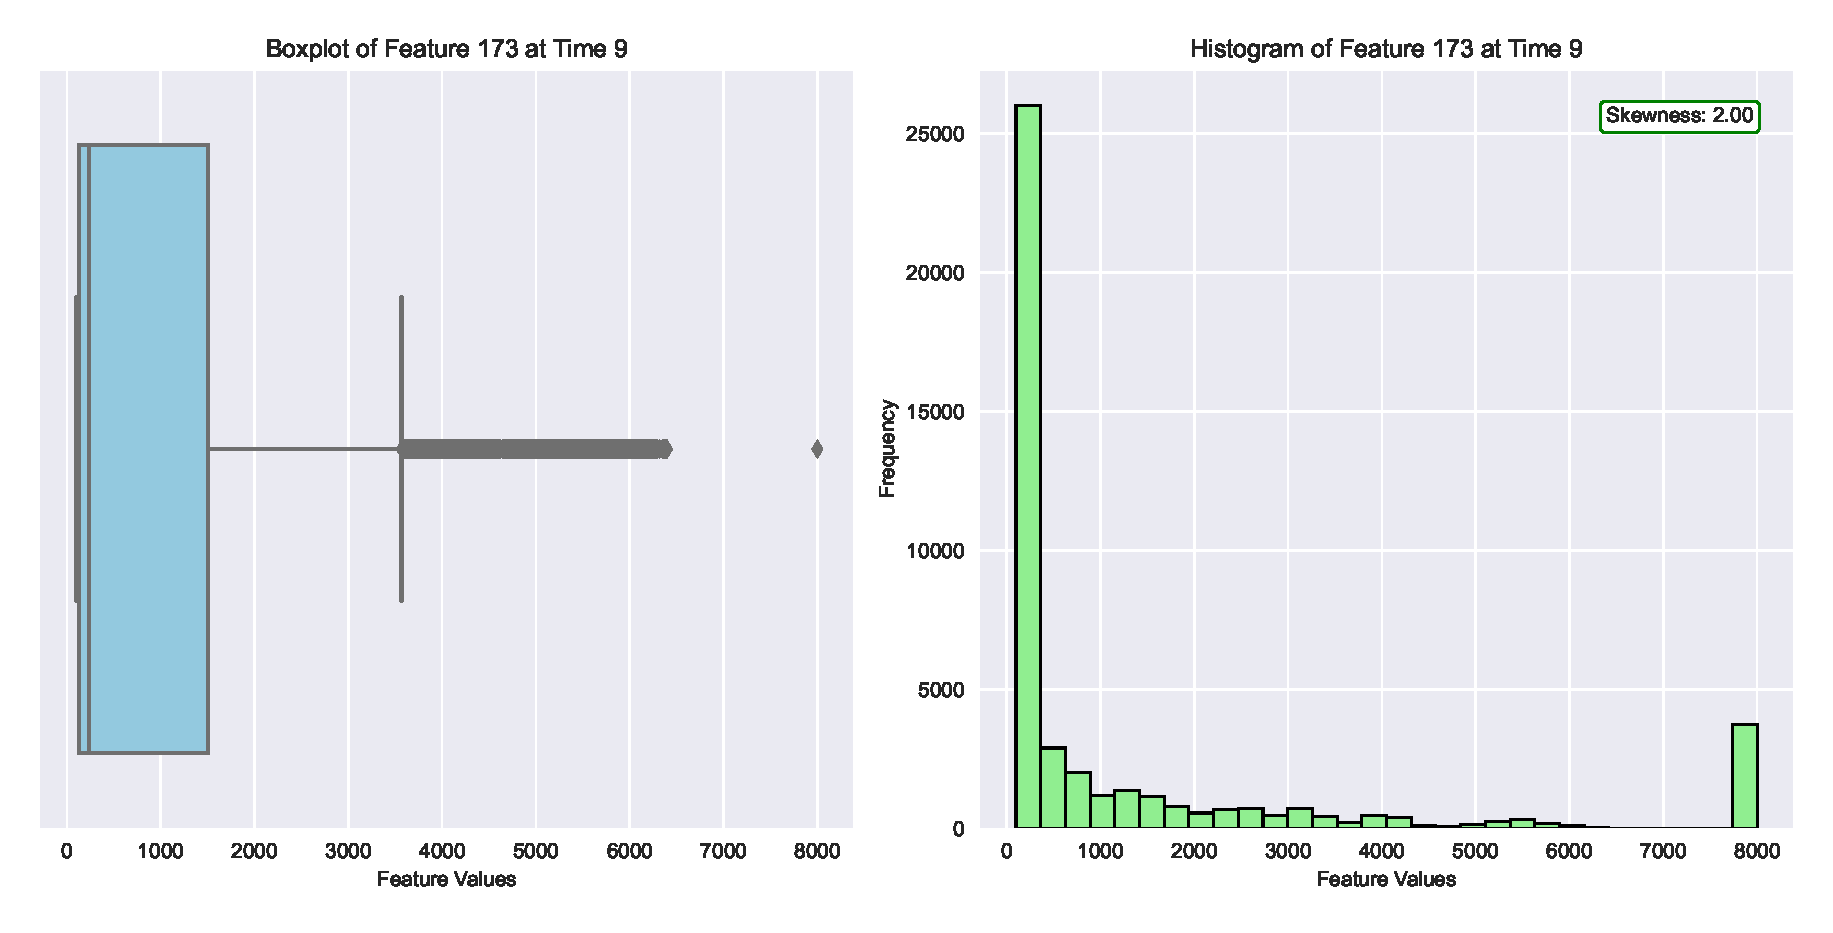
\includegraphics[scale=0.3]{fig/boxplot_histogram_skew}
	\vspace{-0.3cm}
	\caption{Outliers and Skewness $(1.9993748597933172)$.}
	\label{fig:Biases}
	\vspace{-0.1cm}
\end{figure}


\subsubsection{Findings:}

\begin{itemize}
    \item \textbf{Outliers and Anomalies}: Several features, particularly those related to spectral properties such as spectral centroid and rolloff, exhibited outliers. These outliers could indicate recordings that are either mislabeled or possess unique characteristics (e.g., background noise, recording errors) diverging from typical samples.
    \item \textbf{Abnormal Distributions}: Some features showed highly skewed distributions, suggesting the presence of recordings that might not be representative of the dataset's overall characteristics. For instance, features measuring energy and loudness had distributions skewed towards lower values, potentially indicating recordings with very low volume or silence.
    \item \textbf{Potential Mislabelings}: In examining the relationship between features and labels, we noted instances where the feature statistics for certain labels did not align with expectations. This discrepancy could suggest mislabelings, such as a word being incorrectly categorized or background noise being labeled as a speech command.
\end{itemize}

\begin{table}[ht]
  \caption{Feature Analysis by Standard Deviation and Skewness}
  \label{tab:feature_analysis}
  \centering
  \resizebox{\textwidth}{!}{%
  \begin{tabular}{ccccc|ccccc}
    \toprule
    \multicolumn{5}{c|}{Sorted by StdDev} & \multicolumn{5}{c}{Sorted by Skewness} \\
    \cmidrule(r){1-5} \cmidrule(r){6-10}
    Feature ID & Feature Name & Mean & StdDev & Skewness & Feature ID & Feature Name & Mean & StdDev & Skewness \\
    \midrule
        7348 & yin_0 & 1782.25 & 2974.49 & 1.48 & 6997 & power_0 & 13.38 & 148.42 & 72.71 \\
    7523 & yin_0 & 1687.88 & 2930.31 & 1.57 & 6822 & power_0 & 15.28 & 154.51 & 68.48 \\
    173 & yin_0 & 1979.88 & 2929.10 & 1.33 & 697 & power_0 & 18.38 & 179.32 & 52.18 \\
    7173 & yin_0 & 1702.18 & 2912.10 & 1.56 & 6297 & power_0 & 23.72 & 173.67 & 51.19 \\
    348 & yin_0 & 1981.51 & 2896.40 & 1.34 & 522 & power_0 & 16.92 & 171.71 & 47.13 \\
    7698 & yin_0 & 1566.76 & 2857.51 & 1.69 & 6472 & power_0 & 19.78 & 146.62 & 43.24 \\
    523 & yin_0 & 1981.60 & 2853.77 & 1.34 & 7697 & power_0 & 10.69 & 145.80 & 40.68 \\
    6998 & yin_0 & 1629.71 & 2850.66 & 1.64 & 347 & power_0 & 15.64 & 160.70 & 38.76 \\
    698 & yin_0 & 1987.76 & 2810.55 & 1.34 & 872 & power_0 & 20.20 & 167.54 & 35.85 \\
    6823 & yin_0 & 1552.07 & 2779.51 & 1.72 & 7172 & power_0 & 11.59 & 110.97 & 35.20 \\
    \bottomrule
  \end{tabular}
  }
\end{table}

\subsubsection{Implications and Next Steps:}

\begin{itemize}
    \item \textbf{Data Cleaning}: The identified outliers and potential mislabelings necessitate a review and potential cleaning of the dataset to ensure the accuracy of our model. This step may involve reevaluating the labeling process or excluding certain anomalies from the training set.
    \item \textbf{Feature Engineering}: Given the abnormal distributions observed in some features, we may consider feature transformation (e.g., logarithmic transformation) or normalization techniques (e.g., scaling) to mitigate their effects and improve model performance.
    \item \textbf{Further Analysis}: To strengthen our understanding of the data's quality, additional analyses, such as examining feature variance and conducting cluster analysis, could provide further insights into the dataset's structure and any underlying issues.
\end{itemize}

\subsection{Listening and Bias Identification}

Listening to a subset of the recordings has provided valuable insights into the dataset, particularly in terms of accent and gender distribution. These biases could influence model performance and its ability to generalize across different user groups.

\subsubsection{Findings:}

\begin{itemize}
    \item \textbf{Accent Bias}: Analysis of a random sample of approximately 30\% of the data
    revealed a significant bias towards foreign accents, with a ratio of 31 foreign to
    19 domestic (German) accents.
    This imbalance may impact the model’s ability to accurately recognize commands spoken
    with a German accent.
    \item \textbf{Gender Bias}: Another random sample of same size showed a gender distribution of 33 males to 17 females. This skew towards male voices could lead to lower accuracy or performance when recognizing commands from female speakers.
\end{itemize}

%\begin{figure}[!ht]
%	\centering
%	\includegraphics[scale=0.5]{fig/biases}
%	\vspace{-0.3cm}
%	\caption{Biases.}
%	\label{fig:Biases}
%	\vspace{-0.1cm}
%\end{figure}


\subsubsection{Recommendations:}

\begin{itemize}
    \item \textbf{Data Collection}: To mitigate these biases, additional data collection efforts should focus on increasing the number of recordings from female speakers and those with a German accent. This will help in balancing the dataset and improving the model's robustness.
    \item \textbf{Model Training}: Consider using techniques such as stratified sampling\footnote{https://en.wikipedia.org/wiki/Stratified\textunderscore sampling} during training to ensure that the model learns equally well from all categories of data, regardless of accent or gender.
\end{itemize}

\subsection{``Other'' Sounds Analysis}

Listening to some of the sounds labeled as “Other” provided insights into the types of
non-speech audio included in the dataset.
This category is crucial for ensuring the model can appropriately handle irrelevant sounds
when deployed in real-world environments.

\subsubsection{Findings:}

\begin{itemize}
    \item \textbf{Types of Sounds}:
    The "Other" category includes a variety of sounds typically found in household settings,
    such as background noise, household appliances, and television audio.
    These sounds are representative of everyday noises likely to be encountered.
    \item \textbf{Lacking Sounds}:
    In contrast to the relatively broad diversity of the existing sounds, we deem the lack of
    some sounds expectable in a household to be problematic, most notably the absence of child and pet animal sounds.
\end{itemize}

\begin{table}[h]
    \centering
    \caption{Distribution of 'Other' Sounds}
    \label{tab:sounds_distribution}
    {\tiny
    \begin{tabular}{lr}
        \toprule
        Sound Category & Relative Occurrence (\%) \\
        \midrule
        Electronic Device & 16.95\% \\
        Knocking, Thumping & 14.12\% \\
        Vocal Non-Speech & 10.17\% \\
        Rustling (paper, clothes, \ldots) & 9.60\% \\
        Dishes, Bottles & 9.60\% \\
        Walking & 9.60\% \\
        Opening/Closing & 8.47\% \\
        Misc./Unidentifiable & 8.47\% \\
        Liquid & 7.34\% \\
        Engines, Vehicles & 5.65\% \\
        \bottomrule
    \end{tabular}
    }
\end{table}

\subsubsection{Implications:}

\begin{itemize}
    \item \textbf{Data Acquisition}: Refurbishing "Other" sounds with lacking category data is
    essential for providing a broad and representative situative embedding.
    \item \textbf{Model Training}: Training the model to distinguish these "Other" sounds from speech commands is
    essential for preventing false activations and improving user experience.
    The diversity of sounds within this category suggests the need for robust feature extraction techniques that can
    capture a wide range of audio characteristics.
\end{itemize}
